\documentclass{datamade}

%-------Packages---------
\usepackage{tikz}
\usetikzlibrary{shapes,arrows}
\usepackage{setspace}
\usepackage{tikz-cd}
\usepackage[utf8]{inputenc}
\usepackage[all,arc]{xy}
\usepackage{amsthm}
\usepackage{amsrefs}
\usepackage{amsmath}
\usepackage{todo}


%% bold math capitals
\newcommand{\bA}{\mathbf{A}}
\newcommand{\bB}{\mathbf{B}}
\newcommand{\bC}{\mathbf{C}}
\newcommand{\bD}{\mathbf{D}}
\newcommand{\bE}{\mathbf{E}}
\newcommand{\bF}{\mathbf{F}}
\newcommand{\bG}{\mathbf{G}}
\newcommand{\bH}{\mathbf{H}}
\newcommand{\bI}{\mathbf{I}}
\newcommand{\bJ}{\mathbf{J}}
\newcommand{\bK}{\mathbf{K}}
\newcommand{\bL}{\mathbf{L}}
\newcommand{\bM}{\mathbf{M}}
\newcommand{\bN}{\mathbf{N}}
\newcommand{\bO}{\mathbf{O}}
\newcommand{\bP}{\mathbf{P}}
\newcommand{\bQ}{\mathbf{Q}}
\newcommand{\bR}{\mathbf{R}}
\newcommand{\bS}{\mathbf{S}}
\newcommand{\bT}{\mathbf{T}}
\newcommand{\bU}{\mathbf{U}}
\newcommand{\bV}{\mathbf{V}}
\newcommand{\bW}{\mathbf{W}}
\newcommand{\bX}{\mathbf{X}}
\newcommand{\bY}{\mathbf{Y}}
\newcommand{\bZ}{\mathbf{Z}}

%% blackboard bold math capitals
\newcommand{\bbA}{\mathbb{A}}
\newcommand{\bbB}{\mathbb{B}}
\newcommand{\bbC}{\mathbb{C}}
\newcommand{\bbD}{\mathbb{D}}
\newcommand{\bbE}{\mathbb{E}}
\newcommand{\bbF}{\mathbb{F}}
\newcommand{\bbG}{\mathbb{G}}
\newcommand{\bbH}{\mathbb{H}}
\newcommand{\bbI}{\mathbb{I}}
\newcommand{\bbJ}{\mathbb{J}}
\newcommand{\bbK}{\mathbb{K}}
\newcommand{\bbL}{\mathbb{L}}
\newcommand{\bbM}{\mathbb{M}}
\newcommand{\bbN}{\mathbb{N}}
\newcommand{\bbO}{\mathbb{O}}
\newcommand{\bbP}{\mathbb{P}}
\newcommand{\bbQ}{\mathbb{Q}}
\newcommand{\bbR}{\mathbb{R}}
\newcommand{\bbS}{\mathbb{S}}
\newcommand{\bbT}{\mathbb{T}}
\newcommand{\bbU}{\mathbb{U}}
\newcommand{\bbV}{\mathbb{V}}
\newcommand{\bbW}{\mathbb{W}}
\newcommand{\bbX}{\mathbb{X}}
\newcommand{\bbY}{\mathbb{Y}}
\newcommand{\bbZ}{\mathbb{Z}}

%% script math capitals
\newcommand{\sA}{\mathcal{A}}
\newcommand{\sB}{\mathcal{B}}
\newcommand{\sC}{\mathcal{C}}
\newcommand{\sD}{\mathcal{D}}
\newcommand{\sE}{\mathcal{E}}
\newcommand{\sF}{\mathcal{F}}
\newcommand{\sG}{\mathcal{G}}
\newcommand{\sH}{\mathcal{H}}
\newcommand{\sI}{\mathcal{I}}
\newcommand{\sJ}{\mathcal{J}}
\newcommand{\sK}{\mathcal{K}}
\newcommand{\sL}{\mathcal{L}}
\newcommand{\sM}{\mathcal{M}}
\newcommand{\sN}{\mathcal{N}}
\newcommand{\sO}{\mathcal{O}}
\newcommand{\sP}{\mathcal{P}}
\newcommand{\sQ}{\mathcal{Q}}
\newcommand{\sR}{\mathcal{R}}
\newcommand{\sS}{\mathcal{S}}
\newcommand{\sT}{\mathcal{T}}
\newcommand{\sU}{\mathcal{U}}
\newcommand{\sV}{\mathcal{V}}
\newcommand{\sW}{\mathcal{W}}
\newcommand{\sX}{\mathcal{X}}
\newcommand{\sY}{\mathcal{Y}}
\newcommand{\sZ}{\mathcal{Z}}


\renewcommand{\phi}{\varphi}

\renewcommand{\emptyset}{\O}

%--------Theorem Environments--------
%theoremstyle{plain} --- default
\newtheorem{thm}{Theorem}[section]
\newtheorem{cor}[thm]{Corollary}
\newtheorem{prop}[thm]{Proposition}
\newtheorem{lem}[thm]{Lemma}
\newtheorem{conj}[thm]{Conjecture}
\newtheorem{quest}[thm]{Question}

\theoremstyle{definition}
\newtheorem{defn}[thm]{Definition}
\newtheorem{defns}[thm]{Definitions}
\newtheorem{con}[thm]{Construction}
\newtheorem{exmp}[thm]{Example}
\newtheorem{exmps}[thm]{Examples}
\newtheorem{notn}[thm]{Notation}
\newtheorem{notns}[thm]{Notations}
\newtheorem{addm}[thm]{Addendum}
\newtheorem{exer}[thm]{Exercise}

\theoremstyle{remark}
\newtheorem{rem}[thm]{Remark}
\newtheorem{rems}[thm]{Remarks}
\newtheorem{warn}[thm]{Warning}
\newtheorem{sch}[thm]{Scholium}

\newcommand{\action}{\mathbin{\rotatebox[origin=c]{90}{$\circlearrowleft$}}}

\tikzstyle{block} = [rectangle, draw, 
text width=5em, text centered, rounded corners, minimum height=4em]
\tikzstyle{line} = [draw, -latex']

\onehalfspace
\newlength\tindent
\setlength{\tindent}{\parindent}
\setlength{\parindent}{0pt}
\setlength{\parskip}{5pt}
\renewcommand{\indent}{\hspace*{\tindent}}

\bibliographystyle{plain}

%--------Meta Data: Fill in your info------
\title{Modern Approaches to Schema Matching}
\author{Peter Xu (DataMade)}
\begin{document}
	\maketitle
	
\section*{Introduction}

With large collections of data, an analyst often struggles to discover
data that is relevant to the entity of interest. For her to do her
work, the analyst needs to know which datasets could be about her
subject and what the fields in those datasets might mean. \emph{Schema
  matching} attempts to carry out these two task in an automated or
semi-automated way.

More precisely, schema matching addresses two questions.

\begin{itemize}
  \item Which datasets are likely to contain information about the
    same type of entity?
  \item Which fields in separate datasets are likely to contain comparable
    information about an entity?
\end{itemize}

Either problem is difficult by itself, but schema matching is made
even trickier because these questions are entangled. For example, in
order to guess that two columns, from separate tables, are both
referring to a date of birth, we might need know that the rows in each
table are referring to people. Conversely, if we knew that two tables
each had a field that represented a date of birth, we could likely
guess that the rows are about people.

Schema matching has been an extensive subject of academic research.
In this memo, we review that literature and highlight current
approaches to the problems of schema matching and evaluate a number of
open source toolkits. The COMA matcher \cite{coma} will be referred to
often, as it is includes most of of the standard schema matching
techniques.

Throughout this memo we will be talking about tables and columns,
since that is how most of the CARRA data is organized. However, the
field of schema matching encompasses matching data that has
hierarchical or network structure, such as XML data or a database
schema that represents data on an entity across tables. The methods we
describe here apply to that type of data as well.

\section*{Comparing Columns}
Schema matching starts with trying to identify columns that contain
the same type of information. Most modern schema matchers do this by
computing a number of different distance measures for each possible
pair of columns and then applying some rule to aggregate these into a
single score for each column pair. A decision rule is applied to these
scores to decide which column pairs are matches.

\subsection*{Distance Measures}
The distance measures used in schema matching typically are comparing
the names of a column, the contents of a column, and the place of the
column in the structure of the table.

\subsubsection*{String Distance}
Column names can be compared by calculating the distance between the
strings of the column names. The simplest measure is an exact match,
which is $0$ if the strings are exactly the same and $1$ if not.

Beyond that, there are two broad ways of comparing the distance
between strings. The first is to calculate how many insertions,
deletions, or substitutions are required to turn one string into
another. For example, \verb+SCHEMA+ and \verb+SCEMA+ has an distance
of one, because you can transform one string into another with either
a deletion or an insertion.

Alternately, a string can be treated as a collection of characters and
we can calculate the overlap between the collections. A simple measure
of this type is the Jaccard distance

\begin{align*}
\operatorname{J}(A, B) = 1 - \frac{\text{\# Unique Letters
    Common to A and B}}{(\text{\# Unique Letters in A}) +
    (\text{\# Unique Letters in B}) - (\text{\# Unique Letters
      Common to A and B})}
\end{align*}
so that \verb+SCHEMA+ and \verb+SCEMA+ have a Jaccard distance of $0.167$. 

Both approaches have many, many variations, and existing toolkits
usually provide at least four or five to choose from.

\subsection{Semantic Distance}
We would also like to compare the meaning of column names. If column names
were synonyms then there should be little distance between
them. If both column names are examples of common class, for example
\verb+HOURLY WAGE+ and \verb+ANNUAL SALARY+, we would want to score
those as similar, although maybe not as similar as synonyms.

In most modern schema matching toolkits, the semantic distance between
column names are calculated with the aid of dictionaries that list
both synonyms and the class that the word is an example of. Typically,
the semantic distance between two columns names is calculated in the
following way.

\begin{enumerate}
  \item If the words are exactly the same, then the distance is $0$.
  \item If the words are synonyms then, the the distance is $d_1$.
  \item If the words are examples of the same class then the distance
    is $d_2$.
  \item If one word is an example of the second word then the distance
    is $d_3$. For example, \verb+HOURLY WAGE+ and \verb+COMPENSATION+.
\end {enumerate}

The setting of the distances $d_1$, $d_2$, and $d_3$ is typically
arbitrary, with $d_3$ greater than $d_2$ and $d_2$ greater than $d_1$.

The main drawback to the dictionary based approach is that it requires
a domain specific taxonomic dictionary, which is usually laborious to
construct. Available, general purpose taxonomic dictionaries, like
WordNet, do not usually help much in schema matching.

A naive implementation of the dictionary approach will also not be
robust to misspellings or column name abbreviations. This can
addressed with algorithms for approximate string matching used in
spelling correction algorithms. All existing systems seem to have only
implemented the dictionary approach naively.\todo{is that right}

Recent developments in natural language processing suggests a
promising alternative for calculating the semantic distances. The
word2vec model has shown itself to be surprisingly good model for
measuring the ``semantic'' distance between words, and could likely be
usefully applied for schema matching. This technique requires a large
corpus of tables, but does not require a handmade taxonomic
dictionary.\cite{http://radimrehurek.com/gensim/models/word2vec.html}

\subsection*{Data Types}
If we have access to the database system, we can extract metadata on
the types of data that can occur in the columns of table. For example,
we can see whether a column contains integers, floating point numbers,
text, dates, or timestamps. When we compare table columns, we can
compare data types and score columns with the same data types as
similar.

Unfortunately, data often does not have the most specific data type
possible in a database. Timestamps can be represented in
an integer field, integers can be represented in floating point number
fields, and everything can be represented as text. The distance
between timestamp columns should be closer than between text
columns.

\subsection*{Inferring Semantic Meaning}
It is often possible to infer the type of information contained in the
column by examining the data in the column. One method,
described in \cite{regex}, is to develop a library of common formats
(e.g. different ways to write dates/times, email addresses, zip codes,
etc.) described by regular expressions. If columns match the same
formats, then can score them as similar.

This idea could be made more robust by using machine learning
technique for text classification, instead of hand coded, brittle rules.

\subsection*{Distributional Distance}
If two columns contain the same type of information about the same
type of entities, they will often have similar distributions of
data. For example, the distribution of birth dates of unemployment
recipients will be more similar to the distribution of birth dates of
high school freshman than the distribution of application dates for
business licenses, because there will be very few weekends in the
application dates for weekends.

We will often usefully compare distributions by comparing summary
statistics. If we have continuous data, these will likely include

\begin{itemize}
\item Range of Values
\item Average or Median
\item Standard Deviation or Interquartile Range
\item Number of Missing Values
\end{itemize}

If we have categorical data then we can compare

\begin{itemize}
\item All possible values
\item Proportion of categorical values 
\end{itemize}

Alternately, we can compare the distributions directly using
distribution distance measures like the Kullback-Leibler divergence,
the earthmover's distance, or the Chi Squared distance. This can
either be done with the full data, or more practically a representative
sample.

In order to fully benefit from comparing distributions, some care will
be necessary to handle differences in units and coding. If the data is
continuous, float and integer data may need to be standardized. If the
data is categorical, the proportions of the categories should be
compared but the labels of the categories should likely be ignored.

\subsection*{Combining Distances}
Using these distance measures, we will have an array of distances for
every column pair. In order to find the best matches, we need to
combine these multiple measures into a single score.

Modern toolkits allow the user to choose how they want to
aggregate. For example, COMA lets the user decide whether they want
the maximum score, the minimum score, the average score, or a weighted
average score.

All of these approaches potentially discard a lot of information and
also require that each distance measure be normalized to have the same
scale. It would be a much more efficient use of information, and also
simpler, to use the distance measures as features in a statistical
model that predicted whether a pair of columns were about the same
thing or not.

If the distance scores were simply features, then we could remove many
of the arbitrary decisions that we must make within the existing
approach.

For example, instead of choosing how to score the distance between a
timezone datatype and a integer datatype, we could just have a set of
indicator variables that indicate what combination of data types a
pair of columns have. Using logistic regression, or a similar
technique, we would then learn what combinations suggested a good
match or a bad match.

In order to use the machine learning approach, labels are
required. The 





If use more than one type of distance measure, we 


An essential point to remember is that each of these methods outputs a numerical measure of similarity, generally normalized to a number between $0$ and $1$ for later aggregation purposes. For example, methods which simply look for the presence or absence of some feature common to both item labels may have some weight like $0.5$ or $0.7$ assigned to a successful match depending on how significant such a common feature is felt to be; these relative magnitudes may turn out to be significant later depending on the aggregation process used, though not if the measures are reweighted before aggregating (see next section). Thus, there is certainly a fair amount of arbitrariness involved.


\begin{center}
	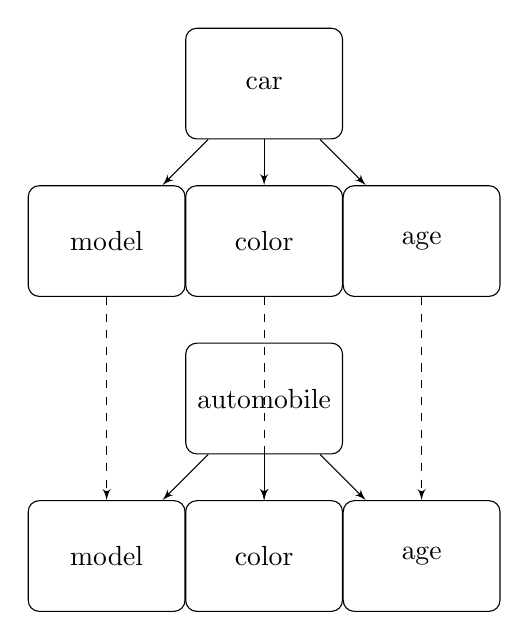
\begin{tikzpicture}[node distance = 2cm, auto]
	% Place nodes
	\node [block] (car) {car};
	\node [block, below of=car] (color) {color};
	\node [block, left of = color] (model) {model};
	\node [block, right of = color] (age) {age};
	\path [line] (car) -- (color);
	\path [line] (car) -- (model);
	\path [line] (car) -- (age);
	
	% Place nodes
	\node [block, below of = color] (automobile) {automobile};
	\node [block, below of=automobile] (color2) {color};
	\node [block, left of = color2] (model2) {model};
	\node [block, right of = color2] (age2) {age};
	\path [line] (automobile) -- (color2);
	\path [line] (automobile) -- (model2);
	\path [line] (automobile) -- (age2);
	
	\path [line,dashed] (color) -- (color2);
	\path [line,dashed] (age) -- (age2);
	\path [line,dashed] (model) -- (model2);
	\end{tikzpicture}
\end{center}

We can determine that ``car'' and ``automobile'' are the same without recourse to semantic methods, purely from the extreme similarity of their children.

Finally, there is measuring similarity based on instances. The obvious way to do this is just by applying an aggregate version of one of the similarity measures like those used for label names. For example, given a method to determine lexicographic similarity between any pair of instances, one can take an average of the similarity scores for the best match over every instance for one (or both) items. \cite{comainstance}

One can also exploit structural features of the instances. One method, described in \cite{regex}, is to develop a library of common formats (e.g. different ways to write dates/times, email addresses, zip codes, etc.) described by regular expressions, and assign higher similarity scores to pairs of items whose items match corresponding regex formats well. In some cases, like database specifications, some of this datatype information is actually encoded in the schema, and so that can simply be used instead.

Given a set of measures to use, a natural way to store all the obtained numerical similarities is in a matrix, in which rows correspond to items from one schema and columns to items from another; each measure then has its own matrix. (Alternately, it can be conceived of as a third dimension of the matrix; hence the term ``similarity cube'' used by \cite{coma}.) Such a matrix might look like the one below with two layers corresponding to two very simple matchers:

\begin{tabular}{|c|c|c|c|c|}
	\hline
LEXICAL & car & color & age & owned by \\\hline
automobile & 0 & 0 & 0 & 0 \\\hline
color & 0 & 1 & 0 & 0 \\\hline
years & 0 & 0 & 0 & 0 \\\hline
owner & 0 & 0 & 0 & 0.6 \\\hline
\end{tabular}

\begin{tabular}{|c|c|c|c|c|}
	\hline
	SEMANTIC & car & color & age & owned by \\\hline
	automobile & 0.9 & 0 & 0 & 0 \\\hline
	color & 0 & 1 & 0 & 0 \\\hline
	years & 0 & 0 & 0.4 & 0 \\\hline
	owner & 0 & 0 & 0 & 0.5 \\\hline
\end{tabular}


Before aggregation, however, often it is useful to do some ``post-processing'' of the similarity matrix, as similarity scores between items can be used in conjunction with other ideas to obtain better measures. For example, if our schemas are directed graphs indicating a hierarchical relation, items/nodes whose children have strong similarity scores should also obtain a boost to their own similarity scores. This is especially relevant if child nodes are the ones with instance data, and so can be analyzed for similarity more thoroughly, since this gives us a way to pass that information back up the tree; see \cite{comainstance}. 

In addition, one may wish to assume transivity in matching; if the edges in a graph representation are bidirectional and indicate some sort of relatedness, matching scores can be propagated in those directions. If one uses an intermediary schema containing already known semantic information, as suggested earlier, this type of propagation can also be used.

\section{Aggregation}

Before aggregating all of the individual similarity scores into actual matches between schema items, one must decide whether one wishes to do a left merge or a total merge. That is, does one want the final schema to essentially be the left schema with as much of the right schema integrated as possible, or a collection of all items in both schemas, with some items identified? The two make sense in different contexts, though the tools we will describe below are not substantially different between them.

\cite{coma} breaks down the progression to selecting matches based on the matrix of similarity scores in a very logical fashion, so I follow them here. 

In the first place, one should calculate an aggregate score for each pair of items, based on all of the match scores (as well as any auxiliary/derived scores, as mentioned at the end of the last section). Conceptually, this is just some sort of measure of center of all of the similarity scores. On one extreme, we can be very risky and take the maximum similarity score; this is almost never a good idea, especially since many of the individual matchers mentioned above are very naive and shallow on their own. On the other, we can be extremely conservative and take the minimum score; this is also usually ill-advised. In between, there are averages of all kinds, the simplest of which would be the classic unweighted mean and median. 

Weighted averages offer more sophistication, and indeed, simply putting weights on matchers based on heuristic estimates of how reliable they are can be useful. Even more effective, however, is the idea of using machine learning. With a relatively small amount user input in the form of some number of true item matches, matching algorithms such as LSD \cite{machine} use the performance of different matchers on this training data to find appropriate weights. (Various algorithms can be used; LSD simply does a least squares regression.) 

To fine tune this further, one could adopt an idea implemented in DataMade's Dedupe algorithm, for the related problem of finding duplicate rows in a database: using the matchers, create an initial model of matches between the schemas, and then solicit input from the user by asking about whether certain items are true matches so as to adjust the weights as efficiently as possible.

Given now a way to obtain aggregate match scores between each pair of items (i.e. having collapsed the third dimension of the similarity cube), it remains to actually select the match candidates. One can require the candidate to be the best match for each item in the first schema, the best item for each item in the second schema, or both, depending on how conservative one wishes to be. In the case of a left merge, of course only the first and the third options make sense.

If one wishes to potentially allow multiple matches, one can use some combination of setting an absolute threshold and choosing top-$n$ matches. An interesting idea from \cite{coma} is to set a threshold relative to the score of the best match, the idea being that multiple matches should occur when there is a group of potential matches which all have close to the same high score.

\section{Evaluation}

With artificially chosen examples of a certain type, evaluation of schema matching can be done in a perfectly standard way. That is, evaluating on schemas which are small and simple enough that objectively correct matches can be given by hand, one can evaluate a schema matcher simply by using the standard measures of precision and recall of automatically detected matches against true matches, inside the space of all possible matches between items.

However, behavior on problems which are larger and more complex may be drastically different than the simple ones for which this is possible; such problems not only may not be feasible to do by hand, but may not have a clear objectively correct set of matches. One would also like to get an idea of how effective a ``real'' application of the matching is, which of course is not hand-verifiable, since otherwise there is no need for the tool. Furthermore, the above discussion on precision/recall applies naturally only to total merges.

To this end, \cite{comabenchmark} outlines some measures which can be used to judge the quality of a matching by means other than accuracy relative to some ``true'' set of matches. Instead, the measures evaluate other aspects of the quality of the merge, based on conceptual understandability and coherence. The essential concepts used are those of coverage, redundancy, compactness.

The \textbf{coverage} of a match refers to what ratio of the total combined items of the original two schemas are represented in the final schema. In cases where the schemas are inheritance-type structures (i.e. represented by directed graphs), particularly when only the bottom-level child items have instance data associated with them like in many databases, one may also consider this ratio restricted to these bottom-level items, since the idea here is that we do not wish to lose information. Of course, this only really makes sense either when we are doing a left merge, or when we are using a match candidate selection technique (see previous section) involving thresholding of some sort; otherwise, of course all the items will be included and the result will always be $1$.

The \textbf{compactness} of a match refers to the ratio of the size of the final merged schema to the sum of the sizes of the two schemas individually. A lower number is desirable because, often, one of the points of the merge is to reduce the schema to a more humanly comprehensible size.

The \textbf{redundancy} of a match applies in cases of inheritance-type directed graph representations; the idea is that one would not like the bottom-level child items to have multiple inheritance paths. Thus, we define it as the ratio between the number of inheritance paths to bottom-level items in the final merged schema to the number of bottom-level items.

Clearly, much like traditional measures such as precision/recall, these measures are designed to have mutual trade-off relationships. For example, coverage and compactness obviously are mutually antagonistic; the only way to obtain both is to match a very high number of items. One can think of redundancy as a measure to prevent just blindly matching many items to achieve good coverage and compactness, since if many of the matches were spurious, almost certainly the non-matching inheritance structures would cause a great deal of redundancy.

\section{Further resources}

It shoudld be noted that the literature on schema matching/ontology merging is vast, and this article did not begin to review it. Instead, aiming at giving an idea of the different steps in how a matching algorithm might be implemented, it largely followed the outline of one particularly flexible matcher (COMA) with many common features. An enormous number of other matchers exist, however, some having completely different sets of features.

A much more comprehensive further resource is \url{ontologymatching.org}, the home page of an organization which hosts academic conferences on the topic. There, one can find much more comprehensive (though often extremely long) surveys, other recent publications, and information on conferences. A subsidiary, the Ontology Alignment Evaluation Initiative, documents online its evaluations of many existing matchers, which may also be of interest.

Finally, listed below are a collection of open-source schema matchers whose licensing, documentation, and source code is all easily accessible online. A brief summary of their basic features is given in the table, though of course each also has many other varying focuses and strengths.

\begin{tabular}{|c|c|c|c|c|c|}
\hline
& COMA 3.0 & OntoBuilder & AgreementMaker & LogMap & S-Match \\\hline
Custom matchers & Yes & Yes & No & No & No \\\hline
Instance data & Yes & Yes & No & No & No \\\hline
Machine learning features & No & No & No & Yes & No \\\hline
Semantic learning features & Yes & No & Yes & Yes & Yes \\\hline
\end{tabular}

These matchers can be found at the following URLs:
\begin{itemize}
\item COMA: \url{http://dbs.uni-leipzig.de/de/Research/coma.html}
\item OntoBuilder: \url{https://bitbucket.org/tomers77/ontobuilder/wiki/OntoM}
\item AgreementMaker: \url{https://agreementmaker.github.io/}
\item LogMap: \url{https://www.cs.ox.ac.uk/isg/tools/LogMap/}
\item S-Match: \url{http://semanticmatching.org/s-match.html}
\end{itemize}

All matchers listed are cross-platform, written in Java, with both command-line and graphical interfaces. They all accept inputs via the standard XML-based format OWL specified by W3C, though other formats are supported by some. 

\begin{thebibliography}{9}
	\bibitem{comasemantic}
	Arnold, Patrick and Rahm, Erhard.
	``Enriching Ontology Mappings with Semantic Relations.''
	University of Leipzig.
	\url{http://dbs.uni-leipzig.de/file/document_0.pdf}	

	\bibitem{coma++}
	Aumuller, David et. al.
	``Schema and Ontology Matching with COMA++.''
	\emph{SIGMOD 2005} (June 2005). 
	\url{http://dbs.uni-leipzig.de/file/comaplusplus.pdf}
	
	\bibitem{coma}
	Do, Hong-Hai and Rahm, Erhard.
	``COMA - A system for flexible combination of schema matching approaches.''
	\emph{Proceedings of the 28th VLDB Conference}, Hong Kong (2002).
	\url{dbs.uni-leipzig.de/file/COMA.pdf}
	
	\bibitem{machine}
	Doan, AnHai et. al.
	``Reconciling Schemas of Disparate Data Sources: A Machine-Learning Approach.''
	\emph{ACM SIGMOD}, Santa Barbara (2001).
	\url{http://homes.cs.washington.edu/~pedrod/papers/sigmod01.pdf}
	
	\bibitem{comainstance}
	Engmann, Daniel and Massmann, Sabine.
	``Instance Matching with COMA++.''
	University of Leipzig.
	\url{ http://dbs.uni-leipzig.de/file/BTW-Workshop_2007_EngmannMassmann.pdf}
	
	\bibitem{ontobuilder}
	Gal, Avigdor and Modica, Giovanni.
	``Onto-Builder: Fully Automatic Extraction and Consolidation of Ontologies from Web Sources.''
	\url{http://ceur-ws.org/Vol-82/SI_demo_04.pdf}

	\bibitem{comabenchmark}
	Raunich, Salvatore and Rahm, Erhard.
	``Towards a Benchmark for Ontology Merging.''
	University of Leipzig.
	\url{http://dbs.uni-leipzig.de/file/E2IN2012-raunich-rahm.pdf}

	\bibitem{regex}
	Zapilko, Benjamin et. al. 
	``Utilizing Regular Expressions for Instance-Based Schema Matching.''
	Leibniz Institute for the Social Sciences.
	\url{http://ceur-ws.org/Vol-946/om2012_poster4.pdf}
\end{thebibliography}
\end{document}
